% Physical Review Research — submission-ready manuscript
% Directed-shortcut first-passage saddle-node. Assembled 2026-06-30.
% BEFORE SUBMISSION: (1) confirm author names/affiliation/order below;
% (2) verify the marked references (% VERIFY); (3) optionally split Fig.1 into 2-3 figures.
\documentclass[reprint,amsmath,amssymb,aps,prresearch,superscriptaddress]{revtex4-2}
\usepackage{graphicx}
\usepackage{bm}
\usepackage{braket}
\usepackage{hyperref}
\graphicspath{{../artifacts/figures/}}

\begin{document}

\title{Saddle-node bifurcation of first-passage-time densities induced by a directed shortcut}

% CONFIRM names/order/affiliation before submission.
\author{Xiaoxiao Zhouyi}
\email{xiaoxiao.zhouyi@bristol.ac.uk}
\author{Luca Giuggioli}
\affiliation{School of Engineering Mathematics and Technology, University of Bristol, Bristol BS8 1TW, United Kingdom}

\date{\today}

\begin{abstract}
First-passage-time (FPT) densities in systems that possess a shortcut to the target are known to be
bimodal: a fast ``direct'' peak and a slow ``indirect'' peak. We show that this bimodality is the
observable-level signature of a \emph{saddle-node bifurcation} that can be solved exactly. Modeling a
directed shortcut to an absorbing target as a rank-one killing defect on a lazy lattice---whose
diffusive limit is Brownian motion on an interval with an interior $\delta$-sink of strength $b$ at
fractional position $\theta$---we show that the second FPT peak is born and annihilated at a fold of a
\emph{signed} spectral mixture, governed by the compact criterion $S_1=S_2=0$, where
$S_n(\tau)=\sum_j G_j\mu_j^{n}e^{-\mu_j\tau}$ and $f'=-S_1$, $f''=S_2$. The double peak exists if and
only if $0<b<b_c(\theta)$, with an explicit boundary $b_c(\theta)$ that is symmetric about
$\theta=\tfrac12$, has a minimum near $\theta\simeq0.381$, and diverges as
$b_c\sim 0.789/\min(\theta,1-\theta)$ near the endpoints; at least three sign-alternating modes are
required, and the fold obeys the universal normal-form scaling
$\tau_+-\tau_-\propto(b_c-b)^{1/2}$, $\Delta f\propto(b_c-b)^{3/2}$. The mechanism is generic rather
than lattice-specific: it follows model-independently from a low-rank non-Hermitian defect, it
generalizes to multiple shortcuts (two shortcuts create a \emph{third} peak organized by a cusp
catastrophe, which we locate), and it survives on a two-dimensional lattice. The threshold $b_c$ is a
time-domain morphology fold, \emph{not} a spectral exceptional point. The result recasts a known
phenomenology as a predictive, exactly solvable bifurcation with a measurable threshold and universal
scaling, testable in feedback-controlled colloidal search and in engineered transport networks.
\end{abstract}

\maketitle

\section{Introduction}
The first-passage time (FPT) to a target is a central observable of stochastic transport, search and
reaction kinetics~\cite{Redner2001,MetzlerBook2014,Benichou2011}. When a searcher has access to a
``shortcut''---a relocation channel, a long-range rewired edge, or an active-transport route---the FPT
density $f(t)$ can become bimodal: fast trajectories that use the shortcut form an early peak, while
slow trajectories that explore the domain form a later peak, provided the two time scales are well
separated~\cite{GodecMetzler2016,Sood2005}. Multimodal capture-time densities are likewise known for
interior partially absorbing traps when several traps are strategically
arranged~\cite{Bressloff2022,Grebenkov2020}, and exact spatiotemporal solutions of confined lattice
random walks with defects are by now a mature program~\cite{Giuggioli2020,MontrollWeiss1965}.

These works \emph{exhibit} multimodality; they do not, however, classify or predict \emph{when} a
second peak exists as a control parameter is varied, nor identify the transition as a bifurcation with
a sharp, computable threshold. Here we supply exactly that. For a minimal directed shortcut---modeled
as a rank-one killing (non-Hermitian) defect---we prove that the birth and death of the second FPT
peak is a \emph{saddle-node} of the density's critical points, give the exact existence boundary
$b_c(\theta)$, a minimal-mode theorem, the universal fold scaling, and demonstrate that the mechanism
is generic (multiple shortcuts, two dimensions). The broad message is that FPT distributions carry
controllable time-domain structure---an emergent arrival-time scale with a threshold---that is
invisible to the mean first-passage time and to spectral gaps.

We are careful to separate what is new from what is not. Shortcut-induced bimodality and interior-trap
multimodality are known~\cite{GodecMetzler2016,Bressloff2022,Grebenkov2020}; the lattice
Green-function/defect method is Giuggioli's~\cite{Giuggioli2020,MontrollWeiss1965}; and
Ref.~\cite{Mattos2012} concerns bimodality of a splitting probability $P(\omega)$, not of $f(t)$. Our
contribution is the exactly solvable \emph{bifurcation-theoretic} account: the fold criterion, the
predictive threshold, and the universality.

\section{Model and exact solution}
Consider a lazy random walk on a ring of $N$ sites: at each step the walker stays with probability
$1-q$ and hops to each neighbor with probability $q/2$. Site $v=0$ is an absorbing target. A directed
shortcut at a source site $u$ diverts probability $\lambda=\beta(1-q)$ from the $u$ self-loop onto the
directed edge $u\to v$. Removing the absorbed state leaves a transient generator on sites
$1,\dots,N-1$ that is a Dirichlet path with a rank-one diagonal killing defect at $u$,
\begin{equation}
Q_b=Q_0-b\,\ket{u}\!\bra{u},
\label{eq:Qb}
\end{equation}
so probability leaks irreversibly from $u$ into the target. Although the shortcut is directed, the
transient block remains symmetric (the directedness enters only the absorption vector), so its
spectrum is real.

The generating function is rational with an exact Montroll-type determinant. With $U_m$ the Chebyshev
polynomials of the second kind, $y=1+(z^{-1}-1)/q$, and $a=q/\lambda$, the characteristic determinant
for a source at $u$ is
\begin{equation}
D_u(y)=a\,U_{N-1}(y)+2\,U_{u-1}(y)\,U_{N-u-1}(y),
\label{eq:Du}
\end{equation}
and the FPT probability is $F(t)=\sum_j B_j s_j^{\,t-1}$ with $s_j=1-q+qy_j$, $D_u(y_j)=0$, and residues
$B_j=q\,\mathcal N_{r,u}(y_j)/D_u'(y_j)$ (Appendix~\ref{app:det}). The antipodal case $u=N/2$ reduces to
$D\propto a\,T_L+U_{L-1}$, recovering the symmetric problem as a special case of the rank-one theory.

\emph{Diffusive limit.} Writing $\theta=u/N$, $b=\beta(1-q)N/q$, $\tau=qt/N^2$ and $s=1-q+q\cos(2w/N)$,
the walk converges to Brownian motion on $[0,1]$ with absorbing ends and an interior $\delta$-sink,
\begin{equation}
\partial_\tau p=\tfrac12\,p_{xx}-b\,\delta(x-\theta)\,p,\qquad p(0)=p(1)=0 .
\label{eq:continuum}
\end{equation}
Its spectrum is fixed by
\begin{equation}
D_\theta(k;b)=k\sin k+2b\,\sin(k\theta)\sin\!\big(k(1-\theta)\big)=0,
\label{eq:Dtheta}
\end{equation}
with $k=2w$ and $\mu_j=k_j^2/2=2w_j^2$; for $\theta=\tfrac12$ this is $\tan w=-2w/b$. The FPT density is
$\Phi_{\xi,\theta}(\tau;b)=\sum_j G_j e^{-\mu_j\tau}$, started at $\xi=r/N$. The \emph{signed}
amplitudes are (Appendix~\ref{app:amp})
\begin{equation}
G_{\xi,\theta}(w)=2w^2\,\frac{\phi_{w,\theta}(\xi)\,I(w,\theta)}{J(w,\theta)},
\label{eq:G}
\end{equation}
where $\phi_{k,\theta}(x)=\sin(k(1-\theta))\sin(kx)$ for $x\le\theta$ and $\sin(k\theta)\sin(k(1-x))$
for $x\ge\theta$, and $I=\int_0^1\phi\,dx$, $J=\int_0^1\phi^2\,dx$ (closed forms in
Appendix~\ref{app:amp}). Modes with $\sin(n\pi\theta)=0$ do not see the sink and contribute the free
term $G_n^{\mathrm{node}}=n\pi[1-(-1)^n]\sin(n\pi\xi)$. We have verified \eqref{eq:G} and the full
master curve against exact finite-$N$ residues to a relative error $\sim10^{-5}$ with clean $O(N^{-2})$
convergence.

\section{The saddle-node existence theorem}
Define the signed spectral moments
\begin{equation}
S_n(\tau;b)=\sum_j G_j\,\mu_j^{\,n}\,e^{-\mu_j\tau},
\label{eq:Sn}
\end{equation}
so that $\Phi'=-S_1$ and $\Phi''=S_2$. An interior extremum of the FPT density is a zero of $S_1$; two
such extrema (a valley--peak pair, i.e.\ the second peak) merge and annihilate at a \emph{saddle-node}
fold,
\begin{equation}
\boxed{\,S_1(\tau_c,b_c)=0,\qquad S_2(\tau_c,b_c)=0\,},
\label{eq:fold}
\end{equation}
with nondegeneracy $S_3(\tau_c,b_c)\neq0$ and $\partial_b S_1(\tau_c,b_c)\neq0$. No positivity is
assumed---the $G_j$ are signed---so this is the correct criterion for a fold of a signed exponential
mixture. Consequently the second peak exists \emph{iff} $0<b<b_c(\theta)$; we verify numerically that
$b_c$ is a \emph{single} fold, i.e.\ the double-peak set is a single connected interval in $b$ with no
re-entrant window.

\emph{Boundary.} $b_c(\theta)$ is symmetric, $b_c(\theta)=b_c(1-\theta)$, with a minimum at
$\theta\simeq0.381$ ($b_c\simeq2.16$) and the endpoint law
\begin{equation}
b_c(\theta)\sim\frac{0.7890261736}{\min(\theta,1-\theta)},\qquad \tau_c\sim0.1579221011\,d^2,
\label{eq:endpoint}
\end{equation}
$d=\min(\theta,1-\theta)$, obtained from a half-line boundary-layer problem. In the antipodal case
$b_c(\tfrac12)=3.0764323604$, with the near-antipodal expansion
$b_c(\tfrac12+\epsilon)=3.0764323604-133.107\,\epsilon^2+O(\epsilon^4)$. Fig.~\ref{fig:main}(a).

\emph{Normal form.} Near the fold the two extrema split as
\begin{equation}
\tau_+-\tau_-\propto(b_c-b)^{1/2},\qquad \Phi(\tau_+)-\Phi(\tau_-)\propto(b_c-b)^{3/2},
\label{eq:scaling}
\end{equation}
the generic saddle-node signature; we confirm both exponents numerically [Fig.~\ref{fig:main}(c)],
which certifies the transition as a fold rather than a spectral crossover.

\emph{Minimal mode count.} A two-mode fold is impossible, even with signs: $S_1=0$ forces
$A_2=-A_1$ ($A_j=G_j\mu_j e^{-\mu_j\tau}$), whence $S_2=(\mu_1-\mu_2)A_1=0$ gives $A_1=A_2=0$. Thus at
least three sign-alternating modes are required; in the antipodal case
$G_1>0,G_2<0,G_3>0,\dots$, and retaining $K$ affected modes gives $b_c^{(3)}=3.046$, $b_c^{(5)}=3.0764$.

\section{Universality}
The fold \eqref{eq:fold} is not special to the ring. For any absorbing Markov generator, a rank-$m$
killing defect $Q_b=Q_0-UBU^\top$ gives, by the Woodbury identity,
\begin{equation}
\det(sI-Q_b)=\det(sI-Q_0)\,\det[I_m+BW(s)],\quad W_{ab}=\bra{u_a}(sI-Q_0)^{-1}\ket{u_b},
\label{eq:woodbury}
\end{equation}
and the FPT density is a signed spectral mixture whose second-peak birth/death is the fold $S_1=S_2=0$.
The double-peak region is an \emph{open} set (structurally stable by the implicit-function theorem),
hence not fine-tuned. The honest universal statement is not ``every shortcut creates a peak'' but
``whenever a shortcut-induced peak is born or annihilated generically, the mechanism is a fold of the
signed spectral mixture.''

\emph{Multiple shortcuts.} For two shortcuts at $\theta_1=\alpha<\theta_2=\beta$ with strengths
$b_1,b_2$, the secular determinant is
\begin{align}
D_{12}(k)={}&k\sin k+2b_1\sin(k\alpha)\sin(k(1-\alpha))\notag\\
&+2b_2\sin(k\beta)\sin(k(1-\beta))\notag\\
&+\tfrac{4b_1b_2}{k}\sin(k\alpha)\sin(k(\beta-\alpha))\sin(k(1-\beta)),
\label{eq:D12}
\end{align}
the last term being a genuine two-defect interaction (it vanishes as the sources coalesce, giving
$b=b_1+b_2$). Two shortcuts can produce a \emph{third} FPT peak: at $(\alpha,\beta,b_1,b_2)=(0.38,0.48,
1.35,0.14)$, $\xi=0.463$, the exact ring shows three peaks at $\tau\simeq3.0\times10^{-4},5.3\times10^{-3},
6.1\times10^{-2}$ [Fig.~\ref{fig:main}(d)]. The triple-peak wedge is organized by a \emph{cusp}
$S_1=S_2=S_3=0$; we locate it at
\begin{equation}
(\alpha,\beta,b_1,b_2,\tau_c)=(0.38,\,0.489580512568,\,1.35,\,1.08389,\,0.0012366),
\label{eq:cusp}
\end{equation}
with $S_4\neq0$ and $\det\partial(S_1,S_2)/\partial(b_1,b_2)=-6.9\times10^7\neq0$, a genuine
codimension-two cusp (Appendix~\ref{app:cusp}). We note that the cusp sits slightly off the
triple-peak example ($\beta\approx0.48958$, not $0.48$, which carries only ordinary folds).

\emph{Two dimensions.} On an $L\times L$ torus with an absorbing target and a directed shortcut, the
same algebra holds [Eq.~\eqref{eq:woodbury} with the lattice resolvent]. Numerically, a single
diffusive peak at $\beta=0$ acquires a shortcut-induced capture peak; the two coexist over a window and
the diffusive peak's prominence falls to zero at $\beta_c^{2D}\simeq0.55$--$0.65$, a fold present at
$L=17,25,33$ [Fig.~\ref{fig:main}(e,f)]. The mechanism is therefore not one-dimensional. A single-site
sink is marginal in 2D (its self-Green function is logarithmically divergent), so the bare $b_c(L)$
drifts as $\sim1/\log L$; the robust, size-independent diagnostics are the moment condition
\eqref{eq:fold} and the fold scaling \eqref{eq:scaling}.

\emph{Robustness.} The fold persists under any perturbation that preserves $S_3\neq0$,
$\partial_b S_1\neq0$: weak hop-rate disorder, small shifts of the source or start, and the laziness $q$
(which merely rescales time, $\tau_c\to\tau_c/q$). It is destroyed only by placing the source on a
symmetry node (dark modes), by source coalescence, or by pushing the start onto the shortcut (the early
peak then escapes to $\tau=0$, outside the interior-fold theorem).

\section{Physical realization and non-Hermitian character}
Physically the shortcut is a localized target-delivery channel: while at $u$ the searcher is delivered
to the target at rate $b$, i.e.\ $f(t)=f_0(t)+b\,p_u(t)$, so a finite gate of width $a$ and local
trigger rate $\kappa$ becomes a $\delta$-sink of strength $\sim\kappa a$. The sharpest realization is
feedback-controlled colloidal or active-particle search: a narrow gate at $x=\theta L$ (optical
tweezers, a microfluidic pulse, or active-particle feedback) that, upon entry, occasionally delivers
the particle to the target and ends the trial; $b$ is the trigger rate, tunable per frame. Repeating
many trials and scanning $b$ at fixed $\theta$ (best near $\theta\simeq0.38$, where $b_c$ is smallest)
should reveal the second peak for $b<b_c(\theta)$ and its annihilation at $b_c$. We caution that
standard resetting-to-origin is \emph{not} this problem---it reinjects probability into the survival
domain; the correct protocol is delivery-and-terminate. A second realization is an engineered or
small-world transport network with a one-way express edge to an absorbing node; two such edges provide
a direct test of the cusp. Intracellular motor capture to a reaction site realizes it in a
coarse-grained (ideally reconstituted) setting.

We stress what the non-Hermitian character is and is not. $Q_b$ is a passive open-Markov loss defect,
analogous to an effective non-Hermitian Hamiltonian with a localized absorber; it is \emph{not}
PT-symmetric (no balanced gain and loss). Crucially, $b_c$ is \emph{not} an exceptional point: an EP
requires eigenvalue coalescence with a defective (Jordan) block, whereas here the eigenvalues remain
real, simple and smooth through $b_c$ (verified), and the fold arises from cancellation among at least
three signed residues. The $(b_c-b)^{1/2}$ scaling in \eqref{eq:scaling} is a saddle-node of the scalar
$f(t;b)$, not EP eigenvalue splitting---the same exponent for a different object. In the reversible
diffusive limit the $\delta$-sink operator is self-adjoint (Sturm--Liouville), so no spectral EP exists.

\section{Discussion}
We have shown that shortcut-induced FPT bimodality, long known phenomenologically, is the observable
signature of an exactly solvable saddle-node bifurcation: a rank-one directed defect produces a second
first-passage peak that exists precisely for $0<b<b_c(\theta)$, is born/annihilated through a fold with
universal $(1/2,3/2)$ scaling, requires at least three sign-alternating modes, generalizes to a cusp
for two defects, and survives in two dimensions. The single most defensible novelty is the
bifurcation-theoretic classification with a predictive threshold, distinct from the known bimodality
and from the underlying defect-resolvent method. The predicted fold exponents and the two-shortcut
triple peak are directly measurable.

Beyond the results proved and verified here, the analysis leaves a small set of technical questions:
a rigorous $N\to\infty$ statement requires, in addition to the standard convergence of fixed-mode
residues (Appendix~\ref{app:amp}), uniform $C^1$ convergence of the moment sums in a neighborhood of
the fold; the large-$L$ renormalized scaling of $b_c$ in two dimensions; and whether the constants
$0.7890\ldots$ and the antipodal $b_c$ admit elementary closed forms.

\begin{acknowledgments}
% CONFIRM funding/acknowledgments before submission.
We thank colleagues at the Bristol Centre for Complexity Sciences for discussions.
\end{acknowledgments}

\appendix

\section{Exact finite-\texorpdfstring{$N$}{N} determinant and residues}\label{app:det}
Deleting the target from the lazy-ring transition matrix leaves the transient block
$Q_0-\lambda\ket{u}\!\bra{u}$ on $\{1,\dots,N-1\}$. Using the matrix-determinant lemma on the rank-one
defect and $\det[yI-\tfrac12 A_{\rm path}]=2^{-(N-1)}U_{N-1}(y)$,
$[\,(yI-\tfrac12A_{\rm path})^{-1}]_{u,u}=2U_{u-1}U_{N-u-1}/U_{N-1}$, one obtains \eqref{eq:Du}. The
piecewise numerator is $\mathcal N_{r,u}=a[A_r+A_{N-r}]+2A_{N-u}[A_r+A_{u-r}]$ for $r\le u$ (and the
mirror for $r\ge u$), $A_m:=U_{m-1}$. The channel (splitting) probability is
$\pi_{\rm sc}(r)=2\min(r,u)[N-\max(r,u)]/(aN+2u(N-u))$, exact by Sherman--Morrison; for the antipodal
case $\pi_{\rm sc}=\rho/(a+L)$. We emphasize $\pi_{\rm sc}$ is the eventual splitting probability, not
the first-peak mass.

\section{Continuum amplitude}\label{app:amp}
With $H_b=-\tfrac12\partial_x^2+b\,\delta_\theta$ and $R_0$ the sink-free interval resolvent, continued
to $z=-k^2/2$, Sherman--Morrison gives
$r_b=r_0-b\,r_0(x,\theta)r_0(\theta,y)/[1+b\,r_0(\theta,\theta)]$, whose poles are the zeros of
\eqref{eq:Dtheta}; the residue eigenfunction is $\psi_j=\phi_{k_j,\theta}$, which satisfies the
$\delta$-sink jump $\psi'(\theta^+)-\psi'(\theta^-)=2b\psi(\theta)\Leftrightarrow D_\theta=0$ (verified
to $2\times10^{-14}$). The absorption density $f=-\tfrac{d}{dt}\!\int p$ has Laplace transform
$\bar f=1-z\bar Q$, and the residue at $z=-\mu_j$ yields $G_j=\mu_j\,\psi_j(\xi)\int\psi_j/\int\psi_j^2$,
i.e.\ \eqref{eq:G}, with
\begin{align}
I(k,\theta)&=\tfrac1k\big[\sin(k(1-\theta))(1-\cos k\theta)\notag\\
&\qquad+\sin(k\theta)(1-\cos k(1-\theta))\big],\\
J(k,\theta)&=\tfrac12[\theta B^2+(1-\theta)A^2]-\tfrac{AB\sin k}{2k},
\end{align}
$A=\sin k\theta$, $B=\sin k(1-\theta)$. The exact identity $J=\sin(k)\,D_k(k;b)/(4b)$ at a root (verified
to $3\times10^{-15}$) links the norm to the determinant derivative and gives nondegeneracy of affected
modes. For $\theta=\tfrac12$, \eqref{eq:G} reduces to
$G_{\xi,1/2}=4w(1-\cos w)\sin(2w\xi)/[\sin^2 w(1+b(b+2)/4w^2)]$. Node modes are the free Dirichlet modes
$\sin(n\pi x)$ at $\sin(n\pi\theta)=0$, with the amplitude quoted in the text. The $I$, $J$ closed forms
match direct quadrature to $10^{-9}$, and the reconstructed master curve matches exact finite-$N$
residues to $\sim10^{-5}$ with $O(N^{-2})$ convergence. Convergence of fixed-mode residues as
$N\to\infty$ follows from norm-resolvent convergence of the killed generator; passing the fold
\eqref{eq:fold} to the limit additionally requires uniform $C^1$ convergence of $S_{1,2,3}$ near
$(\tau_c,b_c)$, which we state as a hypothesis and support by the observed $O(N^{-2})$ fold convergence.

\section{Two-shortcut cusp}\label{app:cusp}
For two sources the rank-two eigenfunction is $\psi_j(x)=-\sum_a b_a c_a^{(j)} r_0(k_j;x,\theta_a)$ with
$c^{(j)}\in\ker[I_2+W(k_j)B]$, and $G_j=\mu_j\psi_j(\xi)\int\psi_j/\int\psi_j^2$ with
$\int\psi_j=-\sum_a b_a c_a I_{\theta_a}$ and $\int\psi_j^2=\sum_{ab} b_a c_a b_b c_b\,C_{ab}$; closed
forms for $I_\theta$ and $C_{ab}$ are elementary. The cusp solves $S_1=S_2=S_3=0$ with $S_4\neq0$ and a
nonzero unfolding Jacobian $\det\partial(S_1,S_2)/\partial(b_1,b_2)$. At \eqref{eq:cusp} an independent
reimplementation gives normalized residuals $\tau S_1/\Phi\approx7\times10^{-12}$,
$\tau^2 S_2/\Phi\approx5\times10^{-11}$, $\tau^3 S_3/\Phi\approx4\times10^{-10}$,
$\tau^4 S_4/\Phi\approx-1.67$, and $\det\partial(S_1,S_2)/\partial(b_1,b_2)\approx-6.9\times10^7$,
confirming a nondegenerate cusp.

\section{Numerical methods and reproducibility}\label{app:numerics}
Exact FPT densities use the symmetric transient block (\texttt{numpy} \texttt{eigvalsh}); high-precision
checks use \texttt{mpmath}. Continuum spectra are the roots of \eqref{eq:Dtheta}/\eqref{eq:D12};
amplitudes use \eqref{eq:G} and Appendix~\ref{app:cusp}. All scripts are deterministic; the figure is
generated by \texttt{dpma\_prr\_figures.py}, the existence boundary by
\texttt{dpma\_saddle\_node\_bc\_theta.py}, the amplitude by \texttt{dpma\_general\_u\_master\_curve.py},
the cusp by \texttt{dpma\_cusp\_verify.py}, and the 2D test by \texttt{dpma\_2d\_universality.py}.

\begin{figure*}
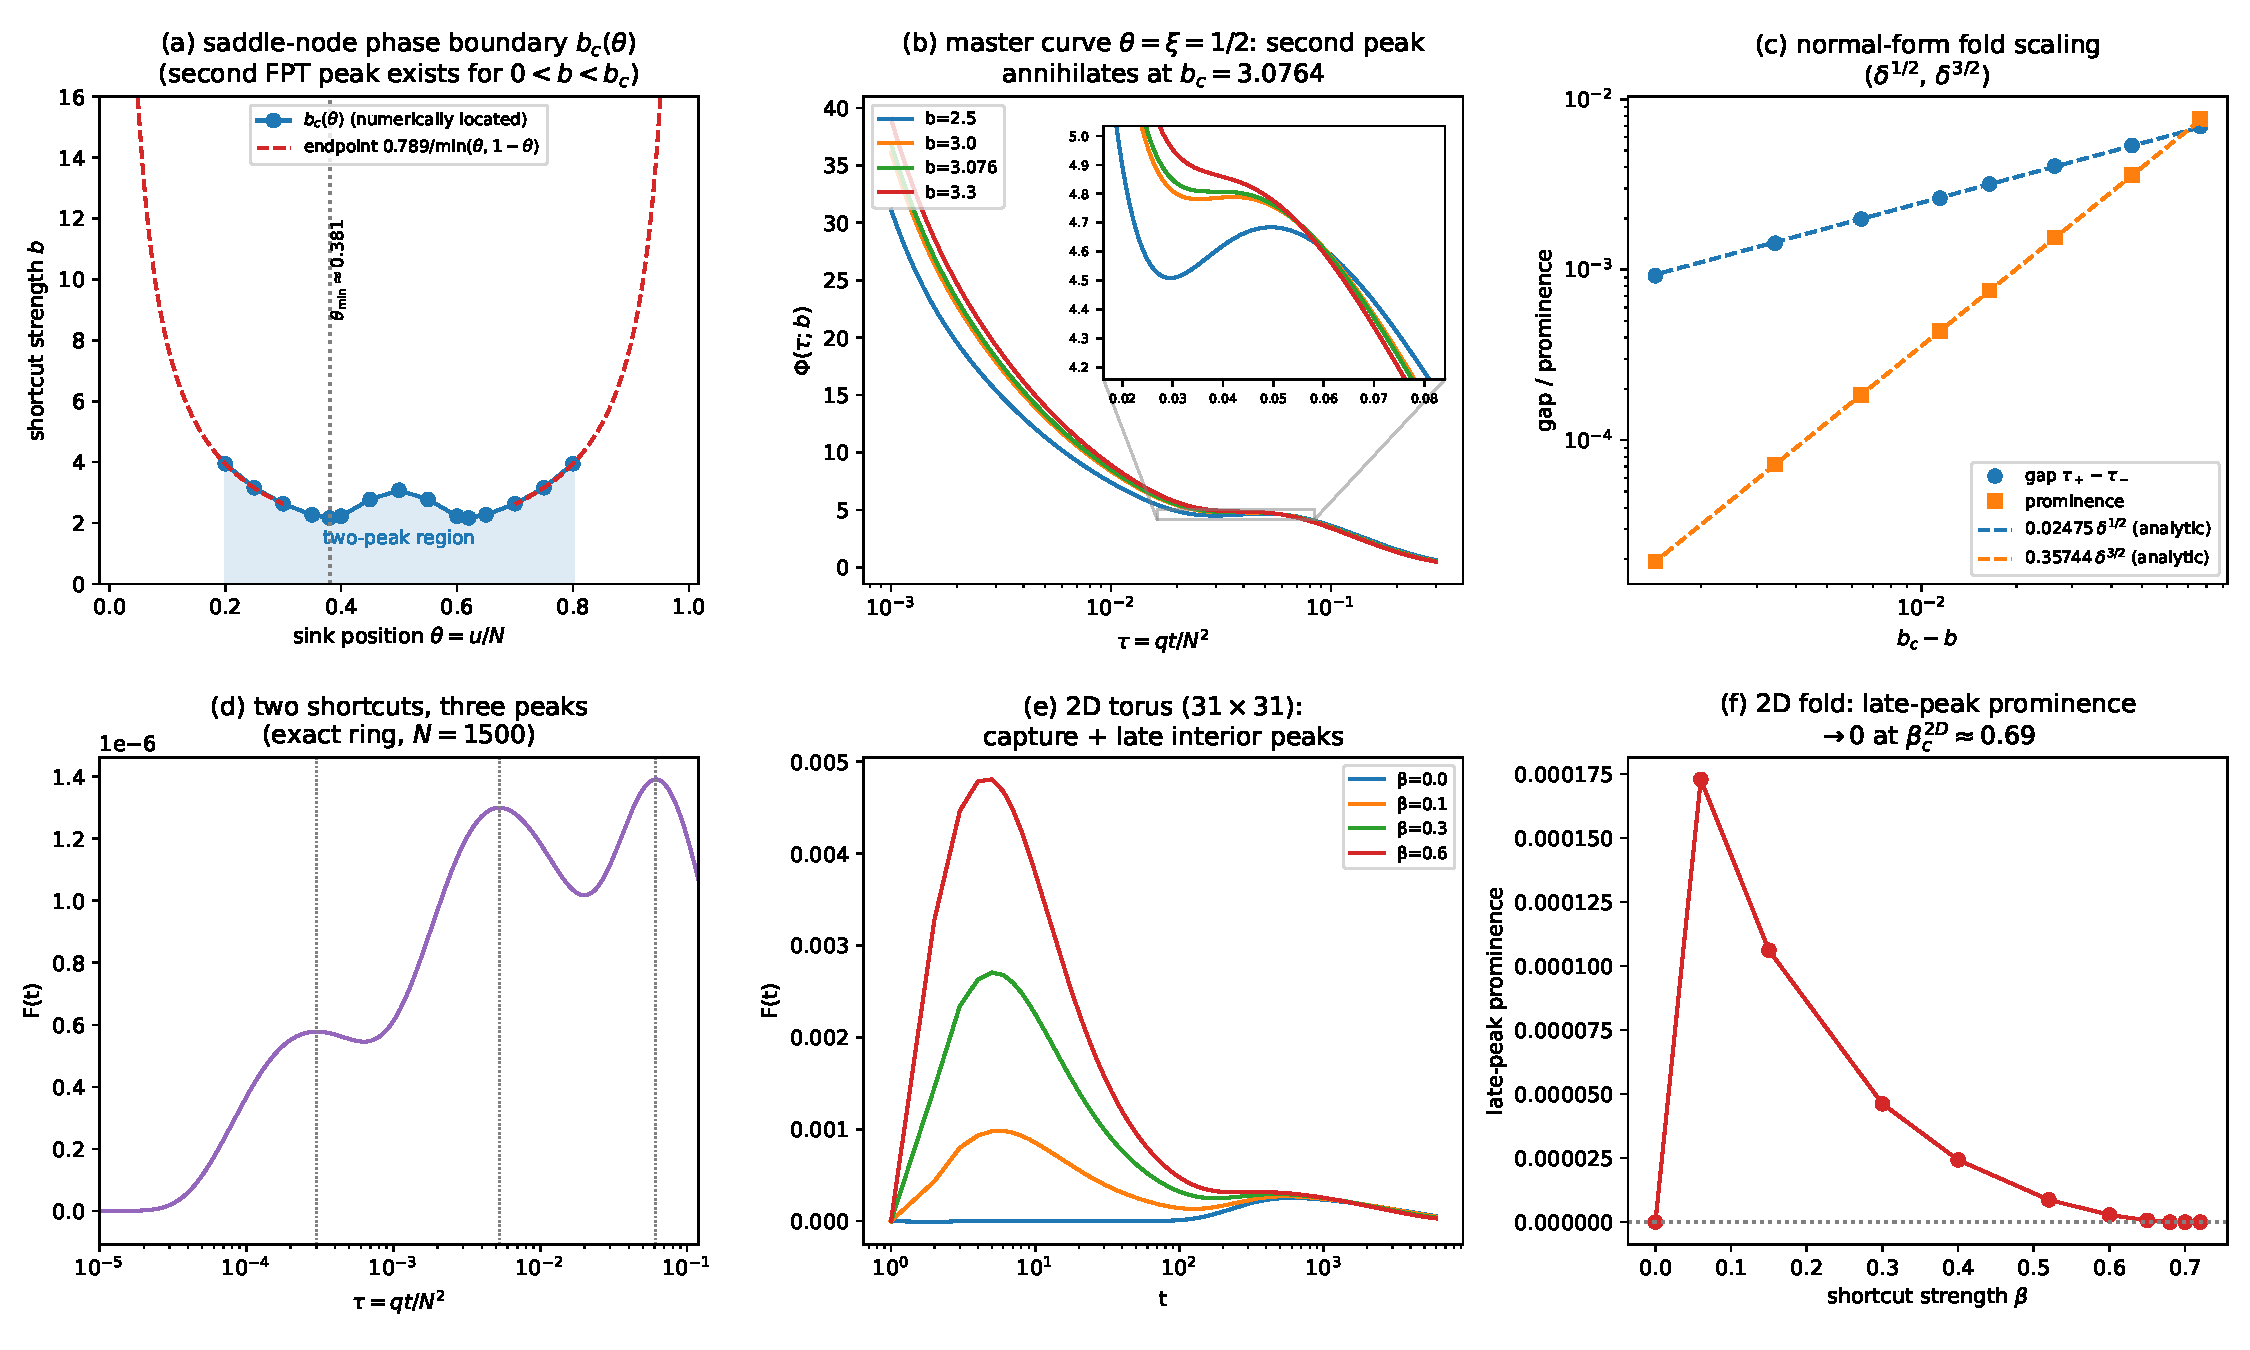
\includegraphics[width=\textwidth]{dpma_prr_figures}
\caption{\label{fig:main}
(a) Saddle-node phase boundary $b_c(\theta)$: the second FPT peak exists for $0<b<b_c(\theta)$;
symmetric, minimum at $\theta\simeq0.381$, with the endpoint law $0.789/\theta$ (dashed).
(b) Master curve $\Phi(\tau;b)$ at $\theta=\tfrac12$ as $b$ crosses $b_c=3.0764$.
(c) Normal-form scaling: gap $\propto(b_c-b)^{1/2}$ and prominence $\propto(b_c-b)^{3/2}$.
(d) Two shortcuts produce a third peak (exact ring, $N=1500$).
(e) 2D torus ($31\times31$): capture and diffusive peaks.
(f) 2D fold: the diffusive-peak prominence vanishes at $\beta_c^{2D}\simeq0.55$--$0.65$.}
\end{figure*}

\begin{thebibliography}{99}
\bibitem{Redner2001} S.~Redner, \emph{A Guide to First-Passage Processes} (Cambridge University Press, 2001).
\bibitem{MetzlerBook2014} R.~Metzler, G.~Oshanin, and S.~Redner (eds.), \emph{First-Passage Phenomena and Their Applications} (World Scientific, 2014).
\bibitem{Benichou2011} O.~B\'enichou, C.~Loverdo, M.~Moreau, and R.~Voituriez, Rev.\ Mod.\ Phys.\ \textbf{83}, 81 (2011). % intermittent search review
\bibitem{MontrollWeiss1965} E.~W.~Montroll and G.~H.~Weiss, J.\ Math.\ Phys.\ \textbf{6}, 167 (1965).
\bibitem{Giuggioli2020} L.~Giuggioli, Phys.\ Rev.\ X \textbf{10}, 021045 (2020).
\bibitem{GodecMetzler2016} A.~Godec and R.~Metzler, Phys.\ Rev.\ X \textbf{6}, 041037 (2016). % VERIFY exact title/vol
\bibitem{Mattos2012} T.~G.~Mattos, C.~Mej\'ia-Monasterio, R.~Metzler, and G.~Oshanin, Phys.\ Rev.\ E \textbf{86}, 031143 (2012).
\bibitem{Sood2005} % VERIFY: small-world / network FPT bimodality reference (e.g. random walks on small-world networks)
E.~Almaas, R.~V.~Kulkarni, and D.~Stroud, Phys.\ Rev.\ E \textbf{68}, 056105 (2003).
\bibitem{Grebenkov2020} D.~S.~Grebenkov, Phys.\ Rev.\ Lett.\ \textbf{125}, 078102 (2020). % VERIFY: partially reactive / boundary local time
\bibitem{Bressloff2022} P.~C.~Bressloff, J.\ Phys.\ A \textbf{55}, 205001 (2022). % VERIFY: encounter-based interior trap
\bibitem{Arnold1992} V.~I.~Arnol'd, \emph{Catastrophe Theory} (Springer, 1992).
\bibitem{Ashida2020} Y.~Ashida, Z.~Gong, and M.~Ueda, Adv.\ Phys.\ \textbf{69}, 249 (2020). % non-Hermitian physics review
\end{thebibliography}

\end{document}
